%% abtex2-modelo-trabalho-academico.tex, v-1.9.7 laurocesar
%% Copyright 2012-2018 by abnTeX2 group at http://www.abntex.net.br/ 
%%
%% This work may be distributed and/or modified under the
%% conditions of the LaTeX Project Public License, either version 1.3
%% of this license or (at your option) any later version.
%% The latest version of this license is in
%%   http://www.latex-project.org/lppl.txt
%% and version 1.3 or later is part of all distributions of LaTeX
%% version 2005/12/01 or later.
%%
%% This work has the LPPL maintenance status `maintained'.
%% 
%% The Current Maintainer of this work is the abnTeX2 team, led
%% by Lauro César Araujo. Further information are available on 
%% http://www.abntex.net.br/
%%
%% This work consists of the files abntex2-modelo-trabalho-academico.tex,
%% abntex2-modelo-include-comandos and abntex2-modelo-references.bib
%%

% ------------------------------------------------------------------------
% ------------------------------------------------------------------------
% abnTeX2: Modelo de Trabalho Academico (tese de doutorado, dissertacao de
% mestrado e trabalhos monograficos em geral) em conformidade com 
% ABNT NBR 14724:2011: Informacao e documentacao - Trabalhos academicos -
% Apresentacao
% ------------------------------------------------------------------------
% ------------------------------------------------------------------------

\documentclass[
	% -- opções da classe memoir --
	12pt,				% tamanho da fonte
	%openright,			% capítulos começam em pág ímpar (insere página vazia caso preciso)
	%twoside,			% para impressão em recto e verso. Oposto a oneside
	a4paper,			% tamanho do papel. 
	% -- opções da classe abntex2 --
	%chapter=TITLE,		% títulos de capítulos convertidos em letras maiúsculas
	%section=TITLE,		% títulos de seções convertidos em letras maiúsculas
	%subsection=TITLE,	% títulos de subseções convertidos em letras maiúsculas
	%subsubsection=TITLE,% títulos de subsubseções convertidos em letras maiúsculas
	% -- opções do pacote babel --
	english,			% idioma adicional para hifenização
	french,				% idioma adicional para hifenização
	spanish,			% idioma adicional para hifenização
	brazil				% o último idioma é o principal do documento
	]{abntex2}

% ---
% Pacotes básicos 
% ---
\usepackage{lmodern}			% Usa a fonte Latin Modern			
\usepackage[T1]{fontenc}		% Selecao de codigos de fonte.
\usepackage[utf8]{inputenc}		% Codificacao do documento (conversão automática dos acentos)
\usepackage{indentfirst}		% Indenta o primeiro parágrafo de cada seção.
\usepackage{color}				% Controle das cores
\usepackage{graphicx}			% Inclusão de gráficos
\usepackage{microtype} 			% para melhorias de justificação
\usepackage{float}
\usepackage{array}
% ---
		
% ---
% Pacotes adicionais, usados apenas no âmbito do Modelo Canônico do abnteX2
% ---
\usepackage{lipsum}				% para geração de dummy text
% ---

% ---
% Pacotes de citações
% ---
\usepackage[brazilian,hyperpageref]{backref}	 % Paginas com as citações na bibl
\usepackage[alf]{abntex2cite}	% Citações padrão ABNT

% --- 
% CONFIGURAÇÕES DE PACOTES
% --- 
\graphicspath{ {images/} } %definindo localização das imagens
% ---
% Configurações do pacote backref
% Usado sem a opção hyperpageref de backref
\renewcommand{\backrefpagesname}{Citado na(s) página(s):~}
% Texto padrão antes do número das páginas
\renewcommand{\backref}{}
% Define os textos da citação
\renewcommand*{\backrefalt}[4]{
	\ifcase #1 %
		Nenhuma citação no texto.%
	\or
		Citado na página #2.%
	\else
		Citado #1 vezes nas páginas #2.%
	\fi}%
% ---

% ---
% Informações de dados para CAPA e FOLHA DE ROSTO
% ---
\titulo{Sistema de Recomendação para Técnicas de Tolerância a Falhas em Ambientes de Nuvem}
\autor{Pedrenrique Gonçalves Guimarães}
\local{São José do Rio Preto, SP}
\data{2019}
\orientador{Aleardo Manacero Junior}
\instituicao{%
  Universidade Estadual Paulista ``Júlio de Mesquita Filho'' (UNESP)
  \par
  Instituto de Biociências, Letras e Ciências Exatas (IBILCE)
  \par
  Departamento de Ciências de Computação e Estatística}
\tipotrabalho{Tese (Graduação)}
% O preambulo deve conter o tipo do trabalho, o objetivo, 
% o nome da instituição e a área de concentração 
\preambulo{Trabalho de Conclusão de Curso (TCC) apresentado como parte dos requisitos para obtenção do título de Bacharel em Ciência da Computação, junto ao Departamento de Ciência da Computação e Estatística, do Instituto de Biociências, Letras e Ciências Exatas da Universidade Estadual Paulista “Júlio de Mesquita Filho”, Câmpus de São José do Rio Preto.}
% ---


% ---
% Configurações de aparência do PDF final

% alterando o aspecto da cor azul
\definecolor{blue}{RGB}{41,5,195}

% informações do PDF
\makeatletter
\hypersetup{
     	%pagebackref=true,
		pdftitle={\@title}, 
		pdfauthor={\@author},
    	pdfsubject={\imprimirpreambulo},
	    pdfcreator={LaTeX with abnTeX2},
		pdfkeywords={abnt}{latex}{abntex}{abntex2}{trabalho acadêmico}, 
		colorlinks=true,       		% false: boxed links; true: colored links
    	linkcolor=blue,          	% color of internal links
    	citecolor=blue,        		% color of links to bibliography
    	filecolor=magenta,      		% color of file links
		urlcolor=blue,
		bookmarksdepth=4
}
\makeatother
% --- 

% ---
% Posiciona figuras e tabelas no topo da página quando adicionadas sozinhas
% em um página em branco. Ver https://github.com/abntex/abntex2/issues/170
\makeatletter
\setlength{\@fptop}{5pt} % Set distance from top of page to first float
\makeatother
% ---

% ---
% Possibilita criação de Quadros e Lista de quadros.
% Ver https://github.com/abntex/abntex2/issues/176
%
\newcommand{\quadroname}{Quadro}
\newcommand{\listofquadrosname}{Lista de quadros}

%\newfloat[chapter]{quadro}{loq}{\quadroname}
\newlistof{listofquadros}{loq}{\listofquadrosname}
\newlistentry{quadro}{loq}{0}

% configurações para atender às regras da ABNT
\setfloatadjustment{quadro}{\centering}
\counterwithout{quadro}{chapter}
\renewcommand{\cftquadroname}{\quadroname\space} 
\renewcommand*{\cftquadroaftersnum}{\hfill--\hfill}

\setfloatlocations{quadro}{hbtp} % Ver https://github.com/abntex/abntex2/issues/176
% ---

% --- 
% Espaçamentos entre linhas e parágrafos 
% --- 

% O tamanho do parágrafo é dado por:
\setlength{\parindent}{1.3cm}

% Controle do espaçamento entre um parágrafo e outro:
\setlength{\parskip}{0.2cm}  % tente também \onelineskip

% ---
% compila o indice
% ---
\makeindex
% ---

% ----
% Início do documento
% ----
\begin{document}

% Seleciona o idioma do documento (conforme pacotes do babel)
%\selectlanguage{english}
\selectlanguage{brazil}

% Retira espaço extra obsoleto entre as frases.
\frenchspacing 

% ----------------------------------------------------------
% ELEMENTOS PRÉ-TEXTUAIS
% ----------------------------------------------------------
% \pretextual

% ---
% Capa
% ---
\imprimircapa
% ---

% ---
% Folha de rosto
% (o * indica que haverá a ficha bibliográfica)
% ---
\imprimirfolhaderosto*
% ---

% ---
% Inserir a ficha bibliografica
% ---

% Isto é um exemplo de Ficha Catalográfica, ou ``Dados internacionais de
% catalogação-na-publicação''. Você pode utilizar este modelo como referência. 
% Porém, provavelmente a biblioteca da sua universidade lhe fornecerá um PDF
% com a ficha catalográfica definitiva após a defesa do trabalho. Quando estiver
% com o documento, salve-o como PDF no diretório do seu projeto e substitua todo
% o conteúdo de implementação deste arquivo pelo comando abaixo:
%
% \begin{fichacatalografica}
%     \includepdf{fig_ficha_catalografica.pdf}
% \end{fichacatalografica}

\begin{fichacatalografica}
	\sffamily
	\vspace*{\fill}					% Posição vertical
	\begin{center}					% Minipage Centralizado
	\fbox{\begin{minipage}[c][8cm]{13.5cm}		% Largura
	\small
	\imprimirautor
	%Sobrenome, Nome do autor
	
	\hspace{0.5cm} \imprimirtitulo  / \imprimirautor. --
	\imprimirlocal, \imprimirdata-
	
	\hspace{0.5cm} \thelastpage p. : il. (algumas color.) ; 30 cm.\\
	
	\hspace{0.5cm} \imprimirorientadorRotulo~\imprimirorientador\\
	
	\hspace{0.5cm}
	\parbox[t]{\textwidth}{\imprimirtipotrabalho~--~\imprimirinstituicao,
	\imprimirdata.}\\
	
	\hspace{0.5cm}
		1. Computação em nuvem.
		2. Tolerância a falhas.
		2. Sistema de recomendação.
		I. Aleardo Manacero Junior.
		II. Universidade Estadual Paulista ``Júlio de Mesquita Filho'' - UNESP.
		III. Departamento de Ciência da Computação e Estatística.
		IV. Bacharelado em Ciência da Computação 			
	\end{minipage}}
	\end{center}
\end{fichacatalografica}
% ---

% ---
% Inserir errata
% ---
%\begin{errata}
%Elemento opcional da \citeonline[4.2.1.2]{NBR14724:2011}. Exemplo:
%
%\vspace{\onelineskip}

%FERRIGNO, C. R. A. \textbf{Tratamento de neoplasias ósseas apendiculares com
%reimplantação de enxerto ósseo autólogo autoclavado associado ao plasma
%rico em plaquetas}: estudo crítico na cirurgia de preservação de membro em
%cães. 2011. 128 f. Tese (Livre-Docência) - Faculdade de Medicina Veterinária e
%Zootecnia, Universidade de São Paulo, São Paulo, 2011.

%\begin{table}[htb]
%\center
%\footnotesize
%\begin{tabular}{|p{1.4cm}|p{1cm}|p{3cm}|p{3cm}|}
%  \hline
%   \textbf{Folha} & \textbf{Linha}  & \textbf{Onde se lê}  & \textbf{Leia-se}  \\
%    \hline
%    1 & 10 & auto-conclavo & autoconclavo\\
%   \hline
%\end{tabular}
%\end{table}
%
%\end{errata}
% ---

% ---
% Inserir folha de aprovação
% ---

% Isto é um exemplo de Folha de aprovação, elemento obrigatório da NBR
% 14724/2011 (seção 4.2.1.3). Você pode utilizar este modelo até a aprovação
% do trabalho. Após isso, substitua todo o conteúdo deste arquivo por uma
% imagem da página assinada pela banca com o comando abaixo:
%
% \begin{folhadeaprovacao}
% \includepdf{folhadeaprovacao_final.pdf}
% \end{folhadeaprovacao}
%
\begin{folhadeaprovacao}

  \begin{center}
    {\ABNTEXchapterfont\large\imprimirautor}

    \vspace*{\fill}\vspace*{\fill}
    \begin{center}
      \ABNTEXchapterfont\bfseries\Large\imprimirtitulo
    \end{center}
    \vspace*{\fill}
    
    \hspace{.45\textwidth}
    \begin{minipage}{.5\textwidth}
        \imprimirpreambulo
    \end{minipage}%
    \vspace*{\fill}
   \end{center}
        
   Trabalho aprovado. \imprimirlocal, %24 de novembro de 2012:

   \assinatura{\textbf{\imprimirorientador} \\ Orientador} 
   \assinatura{\textbf{Renata Spolon Lobato} \\ Convidado 1}
   \assinatura{\textbf{Rodrigo Capobianco Guido} \\ Convidado 2}
   %\assinatura{\textbf{Professor} \\ Convidado 3}
   %\assinatura{\textbf{Professor} \\ Convidado 4}
      
   \begin{center}
    \vspace*{0.5cm}
    {\large\imprimirlocal}
    \par
    {\large\imprimirdata}
    \vspace*{1cm}
  \end{center}
  
\end{folhadeaprovacao}
% ---

% ---
% Dedicatória
% ---

%\begin{dedicatoria}
%   \vspace*{\fill}
%   \centering
%   \noindent
%   \textit{ Inserir dedicatória aqui} \vspace*{\fill}
%\end{dedicatoria}
% ---

% ---
% Agradecimentos
% ---
%\begin{agradecimentos}
%
%
%\end{agradecimentos}
% ---

% ---
% Epígrafe
% ---
\begin{epigrafe}
    \vspace*{\fill}
	\begin{flushright}
		\textit{Epígrafo}
	\end{flushright}
\end{epigrafe}
% ---

% ---
% RESUMOS
% ---

% resumo em português
\setlength{\absparsep}{18pt} % ajusta o espaçamento dos parágrafos do resumo
\begin{resumo}
 A computação em nuvem tem ganhado grande popularidade nos últimos anos por oferecer uma gama de serviços e recursos diversificados de forma rápida, prática e bastante acessível para o público casual e também empresarial. Tais sistemas têm como principais características a escalabilidade e alta carga de trabalho, na maioria dos casos. Entretanto, as plataformas em nuvem também estão bastante suscetíveis a diversos tipos de falhas que podem comprometer o funcionamento dos serviçose e de toda sua infraestrutura, permitindo assim uma perda de dados massiva e possível interrupção de suas atividades por tempo indeterminado. Tais ambientes devem possuir uma boa tolerância a essas falhas, o que significa dizer que a equipe por trás desse ambiente deve ser capaz de identificar e resolver quaisquer falhas de forma a não deixar que estas comprometam o ambiente em questão. Para tratamento de tais falhas, existem diversas técnicas que buscam tratar tais problemas, incluindo uma sistematização em classes com as falhas mais comuns. Para auxiliar administradores desses serviço, este trabalho visa expandir tal sistematização, utilizando um sistema de recomendação inteligente que consiga fazer a sugestão das técnicas corretas para o tratamento de falhas no ambiente de forma automática.

 \textbf{Palavras-chave}: Computação em nuvem, tolerância a falhas, sistema de recomendação.
\end{resumo}

% resumo em inglês
\begin{resumo}[Abstract]
 \begin{otherlanguage*}{english}
   Cloud computing is gaining popularity in recent years for offering a variety of different services and resources in a quick, practical and very accessible way for the casual public and corporations. Such systems have the main characteristics the high scalabilty and workflow, in most cases. However, cloud platforms are also very susceptible to many different types of faults that may compromise the workings of the services and all of its infrastructure, allowing for a massive data loss and also possibly causing an unwanted interruption of its activities for some time. These services should be fault tolerant, which means that any potential failure that may happen during running time should not affect the system, and that the team behind it should be able to identify the problems and solve it without halting the entire operation of the service. There are several techniques available to treat these problems, including a systematic classification of most common faults. To help administrators of these services, this work aims to expand this classification, using an intelligent recommender system that is able to suggest the correct techniques to treat faults automatically.

   \vspace{\onelineskip}
 
   \noindent 
   \textbf{Keywords}: cloud computing, fault tolerance, recommender systems.
 \end{otherlanguage*}
\end{resumo}

% ---
% inserir lista de ilustrações
% ---
\pdfbookmark[0]{\listfigurename}{lof}
\listoffigures*
\cleardoublepage
% ---

% ---
% inserir lista de quadros
% ---
\pdfbookmark[0]{\listofquadrosname}{loq}
\listofquadros*
\cleardoublepage
% ---

% ---
% inserir lista de tabelas
% ---
\pdfbookmark[0]{\listtablename}{lot}
\listoftables*
\cleardoublepage
% ---

% ---
% inserir lista de abreviaturas e siglas
% ---
%\begin{siglas}
%  \item[ABNT] Associação Brasileira de Normas Técnicas
%  \item[abnTeX] ABsurdas Normas para TeX
%\end{siglas}
% ---

% ---
% inserir lista de símbolos
% ---
%\begin{simbolos}
%  \item[$ \Gamma $] Letra grega Gama
%  \item[$ \Lambda $] Lambda
%  \item[$ \zeta $] Letra grega minúscula zeta
%  \item[$ \in $] Pertence
%\end{simbolos}
% ---

% ---
% inserir o sumario
% ---
\pdfbookmark[0]{\contentsname}{toc}
\tableofcontents*
\cleardoublepage
% ---



% ----------------------------------------------------------
% ELEMENTOS TEXTUAIS
% ----------------------------------------------------------
\textual

% ----------------------------------------------------------
% Introdução (exemplo de capítulo sem numeração, mas presente no Sumário)
% ----------------------------------------------------------
\chapter{Introdução}
% ----------------------------------------------------------
A computação em nuvem é uma forma de computação que provê diversos serviços distintos por meio da Internet, de forma que o usuário em questão possa acessar os serviços de qualquer plataforma, desde que possua uma conexão com a Internet. Esse tipo de computação tem se tornado muito popular com a expansão da rede mundial de computadores pelo mundo, e com o pesado investimento em infraestutura proporcionado pelas grandes corporações e operadoras de telecomunicações, que agora tornaram mais acessível ao usuário final o acesso a uma conexão rápida e estável, o que é um requisito fundamental para o correto funcionamento desses serviços.

Gigantes da computação como a Amazon, Google, IBM e Microsoft têm investido pesado em infraestrutura para oferecimento de serviços de computação em nuvem \cite{tsai2010service, lohr2007google}. Outras empresas ganharam grande notoriedade na indústria por oferecerem exclusivamente serviços de computação em nuvem, como é o caso da Netflix, Hulu e Dropbox, por exemplo \cite{berman2012cloud}. 

A alta demanda por tais serviços e modo de operação tem tornado cada vez mais comum o aparecimento de sistemas de computação em nuvem, e cada vez mais profissionais estão sendo treinados para serem capazes de desenvolver e manter tais tecnologias. Entretanto, não diferente de qualquer outro sistema computacional, sistemas de computação em nuvem também são bastante suscetíveis a diversos tipos de falhas e erros que podem comprometer o funcionamento do sistema como um todo. Cada tipo de falha pode ter uma origem diferente, com algum tipo de solução diferente, o que dificulta sua prevenção ou correção, dependendo do tipo de sistema utilizado. Diversos trabalhos na literatura abordam técnicas para lidar com tais falhas e previni-las, e propõem metodologias que visam classificar e identificar as melhores técnicas em casos específicos.

Este trabalho tem o intuito de acrescentar a essas metodologias uma forma de sugestão automática de técnicas de tolerância a falhas por meio de um sistema de recomendação, de forma com que a administração do sistema em questão possa focar na técnica sugerida em vez de buscar diversas soluções distintas que podem resultar em horas infrutíferas de trabalho.

\section{Motivação}

A crescente demanda por serviços baseados em nuvem tem feito o interesse pela área crescer entre os pesquisadores do âmbito da computação para lidar com a tolerância de falhas desses sistemas computacionais. Por consequência, o número de abordagens distintas para suprir tais falhas tem se multiplicado na literatura, e a escolha de abordagens envolve uma série de variáveis que podem levar a dúvidas com relação a qual destes métodos podem ser escolhidos durante uma situação real de risco. Nem sempre a escolha é a melhor possível para uma determinada situação, e uma abordagem pode ter diversos pontos negativos em sua execução.

Levando em conta que sistemas de computação em nuvem devem permanecer operantes de forma ininterrupta, a escolha dos melhores métodos de tolerância a falhas deve ser feita de forma inteligente e deve também estar sujeito a uma rigorosa avaliação por parte da equipe de administração.

\section{Objetivos}

Com o fato de haver inúmeras técnicas distintas para lidar com a tolerância de falhas nesses sistemas, cada uma com suas vantagens e desvantagens, a escolha dessas técnicas pode ser um processo difícil na contenção de falhas.

Utilizando um sistema de recomendação dessas abordagens, os administradores desses sistemas computacionais conseguem, de forma simples, escolher a melhor abordagem para suprir a situação, eliminando a necessidade de uma consulta mais aprofundada, o que, por sua vez, representa uma grande economia de tempo e esforço da equipe de administração.

\section{Organização do texto}

Este documento é dividido em capítulos, seções e diversas subseções. No capítulo a seguir (Capítulo \ref{cap_conceitos}), serão abordados os conceitos básicos necessários para o entendimento do trabalho. Os temas de computação em nuvem, tolerância a falhas e sistemas de recomendação serão analisados e explicados em suas respectivas seções.

Com os conceitos devidamente estabelecidos, o capítulo seguinte (Capítulo \ref{cap_projeto}), expõe as principais propostas para o projeto, com as devidas definições de implementação e detalhes necessários para tal.
% ---
% Capitulo com exemplos de comandos inseridos de arquivo externo 
% ---
\include{abntex2-modelo-include-comandos}
% ---

\chapter{Fundamentação teórica}\label{cap_conceitos}

Como parte essencial para o entendimento do trabalho, este capítulo irá tratar dos principais conceitos e fundamentos necessários para a implementação do projeto de sistema de recomendação.

\section{Computação em nuvem}\label{sec_comp_nuv}

O termo computação em nuvem tem diferentes significados na literatura, e alguns exemplos podem ser mencionados. Em artigo publicado em \citeyear{fernando2013mobile}, \citeauthor{fernando2013mobile} afirmam que consumidores veem computação em nuvem como um serviço padronizado acessível por meio de um aparelho conectado à Internet. Por outro lado, outro artigo de \citeyear{mazhelis2012economic}, \citeauthor{mazhelis2012economic} alegam que profissionais de Tecnologia da Informação veem computação em nuvem como uma \emph{pool} de recursos compartilhados acessados por ambientes computacionais. \cite[p. 1]{khan2018cloud}

De uma forma geral, pode-se representar um exemplo de infraestrutura básica da computação em nuvem como definida na Figura \ref{fig:compnuvem}.

\begin{figure}[h]
	\caption{Exemplo de infraestrutura de computação em nuvem.}
	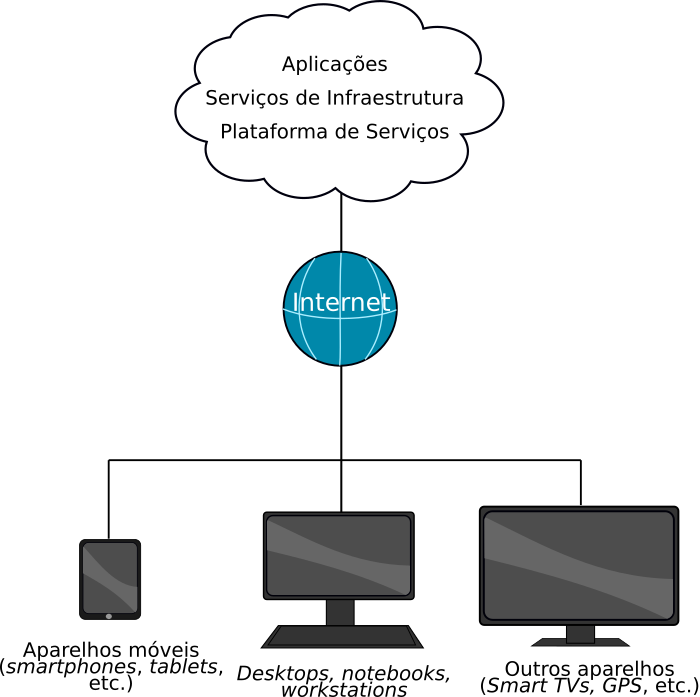
\includegraphics[scale=0.45]{compnuvem}
	\centering
	\label{fig:compnuvem}
	\\
	\centering \textual (Traduzido e adaptado pelo autor \cite{marston2011cloud})
\end{figure}

Em 2011, o \emph{Information Technology Laboratory} (ITL), que faz parte \emph{National Institute of Standards and Technology} (NIST), uma agência governamental que promove a utilização de padrões em ambientes de tecnologia da informação, lançou um documento que define a computação em nuvem como ``um modelo que permite acesso ubíquo, conveniente e sob demanda para uma gama de recursos computacionais compartilhados que podem ser provisionados e liberados com o mínimo de esforço ou interação do provedor de serviço.'' \cite[p. 2]{mell2011nist} (Tradução adaptada pelo autor).

O documento também prevê cinco características essenciais, três modelos de serviço e quatro modelos de implementação que definem o ambiente de computação em nuvem, que serão descritas nas subseções seguintes (\ref{caractessenciais}, \ref{modelosserv}, \ref{modelosimp}).

\subsection{Características essenciais}\label{caractessenciais}

O documento do NIST define as seguintes características essenciais para ambientes de computação em nuvem:
\begin{itemize}
	\item \textbf{Atendimento sob demanda:} O consumidor pode requisitar as operações do serviço em tempo real, como armazenamento de dados por exemplo, sem necessidade de interação humana com o provedor de serviços.
	\item \textbf{Amplo acesso à rede:} Os serviços são disponibilizados por meio do acesso à internet, utilizando mecanismos padronizados que permitam o acesso utilizando diferentes plataformas, como celulares, \emph{notebooks}, \emph{tablets}, \emph{desktops} etc.
	\item \textbf{\emph{Pool} de recursos:} Os recursos computacionais do provedor de serviços deve ser capaz de servir múltiplos consumidores ao mesmo tempo, com diferentes recursos físicos e virtuais sendo destinados dinamicamente de acordo com a demanda do consumidor.
	\item \textbf{Rápida elasticidade:} Os recursos computacionais podem ser fornecidos e liberados de forma elástica, em alguns casos de forma automática, escalando de forma adequada conforme a demanda. Para o consumidor, tais recursos podem parecer ilimitados, ou então podem ser adquiridos em qualquer quantidade a qualquer tempo.
	\item \textbf{Serviços mensuráveis:} Sistemas de nuvem controlam e otimizam automaticamente o uso de recursos utilizando recursos mensuráveis (que geralmente são alcançados utilizando um serviço de ``pagar por uso''). O uso de recursos pode ser monitorado, controlado, e reportado, promovendo transparência tanto para o consumidor quanto para o provedor de serviços.
\end{itemize}

\citeauthor{gong2010characteristics} faz uma relação entre as características de computação em nuvem e computação em grade, um modelo computacional paralela que é baseada em alta performance computacional. Tal comparação está reproduzida na Tabela \ref{tab:comparacao}, de forma traduzida e adaptada.

\begin{table}[H]
    \ABNTEXchapterfont
    \centering
    \caption{Comparação entre Características de Computação em Nuvem e Computação em Grade}
    \begin{tabular}{|c|c|c|}
    \hline
        \textbf{Característica} & \textbf{Computação em nuvem}  & \textbf{Computação em grade}\\
        \hline
        \hline
        Orientada a Serviço & Sim  & Sim\\
        \hline
        Acoplamento Fraco & Sim  & Metade\\
        \hline
        Forte Tolerância a Falhas & Sim  & Metade\\
        \hline
        Modelo de negócios & Sim  & Não\\
        \hline
        Facilmente utilizável & Sim  & Metade \\
        \hline
        Baseado em TCP/IP & Sim & Metade\\
        \hline
        Alta segurança & Metade  & Metade\\
        \hline
        Virtualização & Sim  & Metade\\
    \hline
    \end{tabular}
    \label{tab:comparacao}
\end{table}

Na Tabela \ref{tab:comparacao}, os parâmetros ``sim'' e ``não'' referem-se à presença dessas características especiais nos sistemas, enquanto o parâmetro ``metade'' refere-se a uma presença parcial da característica no sistema computacional. Tal comparação é útil para diferenciar o fato de que Computação em Nuvem não necessariamente significa Computação de Alta Performance, embora muitas vezes estejam associados, e mostra claramente que existem diferenças claras entre os dois modelos computacionais.

Dessa forma, pode-se ver que existem características específicas do modelo de computação em nuvem que são bastante importantes para seu funcionamento.

\begin{itemize}
    \item \textbf{Orientado a serviço:} Serviços de computação em nuvem estão disponíveis para uso sob demanda, como descrito nas características essenciais.
    \item \textbf{Acoplamento fraco:} Ambientes de computação em nuvem utilizam-se de virtualização ou outras tecnologias que separam o lógico do físico. Na seção \ref{sec_arq_comp} isso será um pouco melhor explorado.
    \item \textbf{Forte tolerância a falhas:} Aspecto essencial deste trabalho, existem diversas publicações que mostram a importância da tolerância a falhas na computação em nuvem \cite{jhawar2012fault, ataallah2015fault, amin2015review, cheraghlou2016survey}.
    \item \textbf{Modelo de negócios:} Característica chave que distingue computação em nuvem de computação em grade \cite[p. 278]{gong2010characteristics}. A computação em nuvem é fortemente suportada por grandes companhias na área de Tecnologia de Informação, e todas possuem lucro como principal objetivo do investimento nessas plataformas. Grande parte dos sistemas utiliza alguma forma de pagamento por uso de suas plataformas, e isso os torna sistemas bastante rentáveis para suas respectivas companhias.
\end{itemize}

\subsection{Modelos de serviço}\label{modelosserv}

Os modelos de serviço definidos no documento estão descritos a seguir, com tradução e adaptação pelo autor:

\begin{itemize}
	\item \textbf{\emph{Software as a Service (SaaS)}:} O recurso computacional é disponibilizado para o consumidor como uma aplicação executada em infraestrutura na nuvem. Essa aplicação pode ser acessada de diversos dispositivos, podendo-se utilizar um navegador de internet, ou até mesmo uma aplicação própria. O consumidor, neste caso, não tem nenhum controle sobre os servidores, sistemas operacionais, armazenamento ou aplicações que fazem parte da infraestrutura da rede, limitando-se apenas àquilo que lhe foi designado como serviço disponível.
	\item \textbf{\emph{Platform as a Service (PaaS)}:} O recurso disponibilizado ao consumidor é para a implementação de um sistema de computação em nuvem, podendo assim criar sua prórpia aplicação ou serviço utilizando a infraestrutura existente. Neste caso, o consumidor também não possui controle sobre tal infraestrutura, mas pode implementar aplicações e configurações no ambiente hospedeiro.
	\item \textbf{\emph{Infrastructure as a Service (IaaS)}:} O recurso computacional disponibilizado é prover processamento, armazenamento, rede e outros recursos fundamentais onde o consumidor pode implementar e executar sistemas operacionais e aplicações a seu gosto, quando disponíveis. O consumidor também não controla a infraestrutura, mas já tem controle sobre os sistemas operacionais, armazenamento e aplicações implementadas.
\end{itemize}

\subsection{Modelos de implementação}\label{modelosimp}

Os modelos de implementação mais comuns definidos pelo NIST são os modelos de nuvem privada, nuvem comunitária, nuvem pública e nuvem híbrida. As características de cada um desses serviços está descrita na Tabela \ref{tab:modelos}.

\begin{table}[H]
\ABNTEXchapterfont
\centering
\label{tab:modelos}
\caption{Modelos de Implementação de computação em nuvem}
\begin{tabular}{|m{3.8cm}|m{11.0cm}|}
    \hline
    \multicolumn{2}{|c|}{\centering\textbf{Modelos de Implementação}}\\
    \hline
    \hline
	\centering\textbf{Nuvem privada} & A infraestrutura em nuvem provisionada é de uso exclusivo de uma organização, compondo-se de múltiplos consumidores. \\
	\hline
	\centering\textbf{Nuvem comunitária} & A infraestrutura em nuvem provisionada é de uso exclusivo de uma comunidade específica de consumidores de organizações com interesses em comum.\\
	\hline
	\centering\textbf{Nuvem pública} & A infraestrutura em nuvem provisionada é aberta para o público em geral.\\
	\hline
	\centering\textbf{Nuvem híbrida} & A infraestrutura em nuvem disponibilizada é uma composição de duas ou mais infraestruturas de nuvem descritas anteriormente, que continuam operando de forma independente, mas que se interconectam por uma tecnologia padronizada que permite a portabilidade de aplicações e dados.\\
	\hline
	\end{tabular}
	\textual (Traduzido e adaptado pelo autor)
\end{table}


\subsection{Arquitetura de computação em nuvem}\label{sec_arq_comp}

De uma forma geral, podemos dividir a arquitetura de um sistema de computação em nuvem em quatro camadas \cite{zhang2010cloud}, como também visto na Figura \ref{fig:arqcompnuvem}:

\begin{itemize}
    \item \textbf{Camada de \emph{hardware}:} Responsável por gerenciar os recursos físicos da nuvem, como servidores, roteadores, \emph{switches}, energia e sistemas de resfriamento. Trata-se dos próprios \emph{data centers}.
    \item \textbf{Camada de infraestrutura:} Trata-se da camada de virtualização, que cria a \emph{pool} de armazenamento e recursos computacionais, particionando os recursos físicos usando tecnologias de virtualização.
    \item \textbf{Camada de plataforma:} Consiste no sistema operacional e nos \emph{frameworks} das aplicações. Essa camada facilita a implantação das aplicações executadas.
    \item \textbf{Camada de aplicação:} Consiste nas próprias aplicações executadas em nuvem. Nesses ambientes, as aplicações em nuvem podem ser escaláveis para obter melhor desempenho, acessibilidade e menor custo.
\end{itemize}

\begin{figure}[h]
	\caption{Arquitetura da computação em nuvem.}
	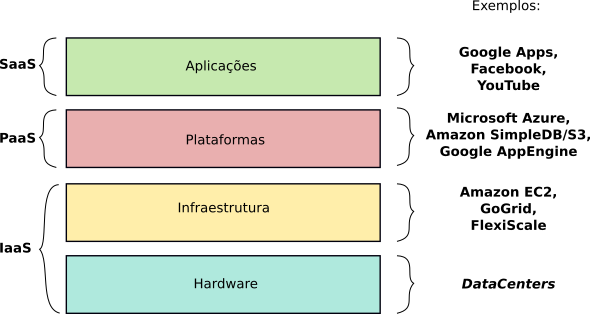
\includegraphics{images/arqcompnuvem.png}
	\centering
	\label{fig:arqcompnuvem}
	\textual (Traduzido e adaptado pelo autor)
\end{figure}

Tal arquitetura torna os serviços de computação em nuvem mais modulares quando comparados a tradicionais \emph{server farms}, por permitir que as camadas funcionem como módulos fracamente conectados entre si, permitindo que esses se expandam e evoluam de forma independente \cite[p. 9]{zhang2010cloud}.

\subsection{Aplicações na indústria}

Existem inúmeras aplicações de computação em nuvem na indústria, que variam de acordo com a natureza da indústria e sua carga de trabalho \cite[p. 10]{khan2018cloud}. Nesta seção, serão apresentados alguns serviços mais conhecidos e relevantes de computação em nuvem, e também serão incluídas algumas aplicações práticas desses serviços em trabalhos publicados, quando disponíveis.

\subsubsection{\emph{Amazon Web Services (AWS)}}

Amazon Web Services (AWS) \cite{aws} é um conjunto de serviços de nuvem, que fornecem computação baseada em nuvem, armazenamento e outras aplicações que atendem tanto o aspecto corporativo quanto a usuários individuais. Nesse ambiente, usuários podem implementar aplicações e serviços sob demanda, pagando de acordo com o uso. \cite[p. 13]{zhang2010cloud}

Neste contexto, a Amazon disponibiliza também o serviço conhecido como \emph{\textbf{Amazon Elastic Compute Cloud}}, também chamado de \textbf{Amazon EC2}. Segundo o próprio serviço: ``O Amazon Elastic Compute Cloud (Amazon EC2) é um web service que disponibiliza capacidade computacional segura e redimensionável na nuvem. Ele foi projetado para facilitar a computação em nuvem na escala da web para os desenvolvedores.'' \cite{amazonec2}. Tal plataforma permite que o usuário administre servidores e \emph{data centers} utilizando APIs ou ferramentas e utilitários disponíveis. As instâncias da EC2 são máquinas virtuais sendo executadas dentro da engine de virtualização Xen \cite{xenengine, zhang2010cloud}.

A estrutura da AWS também comporta serviços como o Amazon Virtural Private Cloud (VPC), que se comporta como uma rede privada virtual (VPN), utilizando os recursos da AWS para permitir uma segurança adicional para o usuário final, com serviços de firewall, detecção de intrusão, entre outros serviços.

Como exemplos do amplo uso desse ambiente computacional em pesquisas práticas, pode-se mencionar trabalhos na área da Biomedicina utilizando computação em nuvem \cite{fusaro2011biomedical}, experimento com sequenciamento genômico chamado \textbf{Globus Genomics} \cite{madduri2014experiences} e análise de performance de computação de alto desempenho \cite{jackson2010performance}. Tais artigos demonstram o potencial crescente de plataformas de computação em nuvem, e demonstram que tais ambientes podem ser utilizados com sucesso em pesquisas importantes, nas quais a obtenção de ferramentas computacionais poderosas próprias é bastante dificultada ou quase impossível.

\subsubsection{Microsoft Azure}

A plataforma Microsoft Azure, antigamente chamada de Microsoft Windows Azure, consiste em uma plataforma da própria Microsoft para executar aplicações e armazenar dados na nuvem \cite{chappell2009introducing}.

Os serviços oferecidos são diversos: armazenamento de dados em nuvem, execução de aplicações, gerenciamento de contâineres, APIs de detecção facial, ferramentas de testes para desenvolvedores, entre outras aplicações \cite{microsoftazure}. 

Os serviços do Microsoft Azure têm sido utilizados em diversas áreas distintas, como geoprocessamento \cite{gong2010geoprocessing}, predição de estruturas de proteínas em 3D \cite{mrozek2015scaling}, utilização de aprendizado de máquina em pesquisa de radiologia \cite{kohli2017implementing}, entre outras tantas aplicações disponíveis na literatura.

\subsubsection{Dropbox}

Criado em 2007, o serviço conhecido como Dropbox \cite{dropbox} ocupa um nicho específico no ramo de computação em nuvem. Seu principal modelo de negócio é o armazenamento de dados em nuvem, oferecendo serviços para corporações e para usuários finais. Ele oferece aos usuários um serviço gratuito de armazenamento de até 2 GB por usuário. Esse montante pode ser expandido em até 3 TB ou mais mediante pagamento de planos específicos, que oferecem recursos adicionais como sincronização automática com dispositivos conectados, busca em texto, recuperação de arquivos desejados e suporte dedicado \cite{dropboxplans}.

\subsubsection{Google App Engine}

A Google App Engine é mais um dos serviços de computação em nuvem da Google. Consiste em uma plataforma para criação de aplicativos de forma escalonável, totalmente gerenciada e sem servidor. Na plataforma pode-se utilizar linguagens e frameworks populares como Java, PHP, Node.js, Python, C\#, .Net, Ruby e Go, ou o usuário pode também utilizar seu próprio framework sobre a plataforma \cite{googleapp}.

O serviço conta também com ferramentas para contâiners, controle de versão, segurança com certificados gerenciados SSL/TLS, ferramentas para depuração, dentre tantas outras opções para desenvolvedores.

\section{Tolerância a falhas}

O uso de sistemas computacionais é ubíquo no mundo moderno, extendendo-se a aplicações em sistemas de defesa, sistemas aéreo, controle de tráfego aéreo, sistemas bancários, jogos virtuais, dentre tantos outros. A variedade de aplicações e a importância crescente desse setor trouxe à tona a confiabilidade de sistemas computacionais para as mais diversas aplicações \cite{andersonfault}.

Um exemplo de preocupação com o funcionamento adequado desses sistemas ocorreu no fim da década de 1990, quando percebeu-se o modo ineficiente de armazenamento e formatação de datas de calendários em sistemas computacionais da época, e que colocaria em risco a correta execução de milhares de serviços dependentes desses sistemas, podendo também ocasionar uma pane geral de alguns sistemas de alto risco. Tal episódio é conhecido na literatura como ``Problema do Ano 2000'', muitas vezes estilizado como ``Y2K \emph{problem}'', ou popularmente chamado de ``\emph{Bug} do Milênio'' . A preocupação com uma pane em massa de praticamente todos os sistemas computacionais levou a criação de uma série de medidas para garantir a correção desse problema nos sistemas existentes e prevenir a ocorrência de problemas similares em futuros sistemas desenvolvidos \cite{petersen1998y2k}.

Este clássico exemplo de prevenção de falhas mostra uma fraqueza de alguns sistemas computacionais em lidar com falhas previstas anteriormente. Caso tais correções e recomendações não fossem consideradas, especula-se que as consequências poderiam ser catastróficas para os mais diversos setores que dependiam desses sistemas computacionais \cite{smith1997year}. Assim sendo, deve-se levar em consideração que existem problemas aos quais sistemas computacionais estão sujeitos, mas que podem ser tratados adequadamente em tempo de execução, evitando ao máximo comprometer o funcionamento desse sistema.

\subsection{Conceitos básicos}

Assim como os sistemas mencionados anteriormente estavam sujeitos a falhas causadas por uma falta de planejamento dos desenvolvedores, sistemas computacionais modernos também estão sujeitos a inúmeros tipos de falhas, que podem fugir completamente ao controle tanto de administradores do sistema quanto aos desenvolvedores ou fabricantes de tal produto.

Uma falha no sistema ocorre quando o serviço oferecido se desvia do serviço especificado, na qual o serviço especificado significa uma descrição coerente do que é esperado desse serviço \cite{laprie1985dependable}. Nesse contexto, pode-se afirmar que ocorreu um erro, decorrente de uma falha. Isto é, o erro é uma manifestação de uma falha no sistema, e a falha é a manifestação do erro no serviço \cite{laprie1985dependable}.

O conceito de tolerância a falhas em computação é bastante antigo e se aplica tanto no âmbito do fabricante de \emph{hardware} quanto na área de desenvolvimento de \emph{software} \cite{randell1975system}. Para ambos, é importante garantir a confiabilidade do sistema para qualquer um que venha a utilizá-lo posteriormente. Isso quer dizer que o sistema deve garantir que, mesmo após a ocorrência de algum tipo de falha, não ocorra interrupções no serviço \cite{bala2012fault}.


\subsection{Modelos de falhas}



\subsection{Técnicas de tolerância a falhas}

\subsubsection{Técnicas reativas}

\subsubsection{Técnicas proativas}

\subsection{Sistematização}

\subsection{Aplicações}



% ---

% ---
\section{Sistemas de recomendação}\label{sec_recom}

Parte essencial de vários sistemas computacionais hoje em dia, sistemas de recomendação estão cada vez mais presentes na vida dos usuários de redes sociais e de usuários casuais de internet. Esses sistemas estão muitas vezes presentes de forma imperceptível, e podem ser partes fundamentais do modelo de negócio de várias companhias.

Nesta seção, serão apresentados os conceitos básicos dos sistemas de recomendação, suas abordagens mais conhecidas e aplicadas, bem como exemplos práticos de sua aplicação em situações do cotidiano.

\subsection{Conceitos básicos}

Sistemas de recomendação são um conjunto de técnicas e ferramentas que fornecem sugestões de itens que podem ser úteis para o usuário final \cite{resnick1997recommender, good1999combining, burke2007hybrid}. Amplamente utilizados na indústria de computação e no mercado em geral, sistemas de recomendação têm ganhado notoriedade entre grandes empresas de comércio virtual, redes sociais e serviços de computação em nuvem, pela capacidade de entregar ao consumidor ou usuário final uma experiência personalizada e intuitiva com sua aplicação.

Em meio à popularidade e relevância desse tipo de sistema na indústria, um dos casos mais populares de incentivo à pesquisa desse tipo de sistema ocorreu no episódio conhecido como ``\textbf{Prêmio Netflix}'' (em inglês: \emph{Netflix Prize}), ocorrido em outubro de 2006, quando a Netflix \cite{netflix} lançou um banco de dados contendo 100 milhões de avaliações anônimas de 18.000 filmes, feitas por 480.000 usuários e desafiou a comunidade de cientistas da computação, pesquisadores de aprendizado de máquina e pesquisadores de \emph{data mining} a desenvolver sistemas que conseguiriam superar seu próprio sistema de recomendação, conhecido como \emph{Cinematch} \cite{bennett2007netflix}. O prêmio dessa competição era 1 milhão de dólares para a equipe vencedora, o que certamente chamou a atenção de muitos pesquisadores ao redor do planeta. Tal episódio gerou uma situação sem precedentes na história de pesquisa na área de filtragem colaborativa \cite{bell2007lessons}. Em menos de um ano, mais de 20.000 times de 152 países diferentes haviam se registrado, sendo que desses apenas 2.000 haviam submetido seu conjunto de previsões até Junho de 2007 \cite{bennett2007netflix}. O prêmio final foi dado em 2009 para o time de pesquisa do \emph{AT\&T Labs}, chamado de \textbf{BellKor}, que havia conseguido resultados cerca de 10,10\% melhores que o \emph{Cinematch} \cite{koren2009bellkor}.

Existem inúmeras razões que levam empresas e provedores de serviços como a Netflix a explorar e melhorar esse tipo de sistema, as quais estão listadas a seguir \cite{ricci2011introduction}:

\begin{itemize}
    \item \emph{Aumentar o número de itens vendidos:} Uma das funções mais importantes de Sistemas de Recomendação comerciais é ser capaz de vender itens adicionais aos escolhidos por consumidores. Os itens recomendados geralmente se adequam ao perfil de compra do usuário, e por isso são mais prováveis de serem comprados pelo mesmo enquanto pesquisa algo relevante. Aplicações não-comerciais também possuem os mesmos objetivos, mesmo que não haja um custo envolvido para o usuário ao selecionar um item.
    \item \emph{Vender itens diversificados:} Um sistema de recomendação também deve ser capaz de permitir que o usuário selecione itens que possivelmente sejam mais difíceis de encontrar sem uma recomendação precisa. Por exemplo, ao pesquisar um filme na plataforma da Netflix, um usuário irá se deparar com títulos semelhantes em conteúdo, que possuem temática similar ao procurado, mas que geralmente são menos populares. Essa é uma forma de promoção desses títulos menos populares.
    \item \emph{Aumentar a satisfação do usuário:} Um sistema de recomendação bem projetado pode melhorar a experiência do usuário com a aplicação. O usuário encontrará recomendações interessantes, relevantes e, com uma boa interação humano-computador, também irá apreciar a utilização do sistema.
    \item \emph{Aumentar a fidelização do usuário:} Usuários tendem a se tornar mais fiéis a um determinado \emph{Web site} que, ao ser visitado, reconhece o consumidor e o trata como um visitante valioso, personalizando a experiência do usuário com aquele serviço. Consequentemente, quanto mais o usuário utiliza o serviço, mais refinadas são as recomendações do sistema, e melhor é a representação de suas necessidades naquele sistema.
    \item \emph{Melhor entendimento dos desejos do usuário:} Conectando com o ponto anterior, o entendimento do perfil do consumidor ou usuário é um importante aspecto de um sistema de recomendação. A previsão de desejos do usuário pode ser utilizado pelo provedor de serviço para inúmeros outros objetivos, como por exemplo melhor gerenciar o estoque de determinados itens ou produção, ou personalizar a experiência de outros usuários com gostos similares.
\end{itemize}

Como visto anteriormente, é importante que sistemas de recomendação coletem diversos tipos de dados para construir suas recomendações \cite{ricci2011introduction, herlocker2004evaluating}, para que dessa forma o sistema consiga fazer uma previsão de algo desejado pelo usuário final. Alguns desses dados podem ser coletados do histórico de outros usuários, ou por um banco de dados pré-estabelecido. Dependendo da abordagem utilizada, o número de informações contidas no banco de dados pode ser crucial para refinar as recomendações do usuário \cite{resnick1997recommender}.

\subsection{Modelos}

Existem alguns modelos de sistemas de recomendação trabalhados na literatura. De uma forma simplificada, podemos classificá-los em três abordagens distintas, como visualizado na Figura \ref{fig:sisrec}. As abordagens mais comuns são: \textbf{Filtragem Colaborativa}, \textbf{Baseada em Conteúdo} e \textbf{Híbrida} \cite{ricci2011introduction}.

\begin{figure}[H]
    \centering
    \caption{Modelos de sistemas de recomendação}
    \includegraphics[width=16.0cm,height=7.0cm]{images/sisrecomendacao.png}
    \label{fig:sisrec}
    \\
    \textual (Traduzido e adaptado pelo autor, de Wikimedia Commons)
\end{figure}

Dentre esses modelos mencionados, o mais popular e mais presente na literatura é o sistema de recomendação de filtragem colaborativa \cite{ricci2011introduction, isinkaye2015recommendation, good1999combining}, por sua maturidade e robustez de desenvolvimento, e por sua ampla aplicação e métodos de implementação. Como visto na Figura \ref{fig:sisrec}, existem diferentes formas de implementação de um sistema de recomendação de Filtragem Colaborativa, que serão exploradas nas subseções seguintes.  

Existem também outras abordagens citadas na literatura, algumas até derivadas da filtragem colaborativa, como por exemplo recomendação baseada em contexto \cite{adomavicius2011context}, baseada em comunidade e baseado em conhecimento \cite[p. 13]{ricci2011introduction}. Algumas dessas abordagens ainda não apresentam um grau de maturidade tão avançado quando o método de Filtragem Colaborativa e, portanto, neste trabalho serão apenas apresentadas as técnicas mais comumente utilizadas e mais bem trabalhadas na literatura.

\subsubsection{Filtragem Colaborativa}

Trata-se do modelo de sistema de recomendação mais trabalhadas na literatura, também reconhecida como uma das mais promissoras tecnologias da área \cite{isinkaye2015recommendation, resnick1997recommender, schafer1999recommender}, a filtragem colaborativa funciona por meio da construção de um banco de dados de preferências de itens por usuário \cite{sarwar2002recommender}. Quando um novo usuário entra no sistema, tal usuário é comparado com outros do banco de dados para descobrir \emph{vizinhos}, que historicamente possuem gostos similares a ele.

A Filtragem Colaborativa é o processo de filtragem de informação ou padrões utilizando técnicas de colaboração entre múltiplos agentes, pontos de vista, fontes de dados, etc \cite{terveen2001beyond}. Aplicações que utilizam filtragem colaborativa geralmente envolvem grandes bancos de dados.

Para definir as recomendações, os usuários devem avaliar os itens \cite{herlocker2004evaluating} para que esses sejam posteriormente sugeridos para outros usuários vizinhos no banco de dados. O funcionamento simplificado desse modelo está ilustrado na Figura \ref{fig:collabfilt}.

\begin{figure}[H]
    \centering
    \caption{Diagrama do funcionamento da Filtragem Colaborativa}
    \includegraphics[width=16.0cm,height=13.0cm]{images/collabfilt.png}
    \label{fig:collabfilt}
    \textual (Traduzido e adaptado pelo autor, de Wikimedia Commons)
\end{figure}

\subsubsection{Recomendação Baseada em Conteúdo}

\subsubsection{Recomendação Híbrida}

\subsection{Aplicações}

O uso de tecnologias de recomendação é bastante presente em plataformas de computação em nuvem, e mostram-se bastante eficazes na arte de influenciar o usuário final a tomar uma decisão baseada naquilo que lhe é sugerido \cite{shani2011evaluating}. O uso de um sistema de recomendação varia de acordo com o modelo de negócio utilizados e sua plataforma necessária para funcionamento. As pesquisas em sistemas de recomendação são feitas com ênfase principalmente nas aplicações comerciais, já que, sem desemerecer suas contribuições teóricas, há uma preocupação em melhorar sua praticidade comercial \cite{ricci2011introduction}.

Sistemas como esse também são amplamente utilizados na área do comércio virtual, mais conhecido como \emph{e-commerce} \cite{sarwar2002recommender}, fazendo a sugestão de produtos e anúncios para usuários que demonstram interesses em determinadas categorias pela internet. De uma forma geral, podemos descrever o uso prático de sistemas de recomendação nas seguintes áreas \cite{ricci2011introduction}:

\begin{itemize}
    \item \textbf{Entretenimento:} recomendações de filmes, séries, desenhos, músicas, jogos.
    \item \textbf{Conteúdo:} jornais personalizados, recomendação de documentos, livros, páginas \emph{web}, aplicações em aprendizado a distância, fitros de \emph{e-mails}.
    \item \textbf{E-commerce:} recomendação para consumidores para comprar produtos como livros, câmeras, computadores etc.
    \item \textbf{Serviços:} recomendação de serviços de viagens, recomendação de experts para consultas, recomendação de casas para alugar, ou serviços que combinem duas pessoas, como um aplicativo de encontros, ou até mesmo sugestão de oponentes em algum jogo.
\end{itemize}

Neste contexto, serão abordados neste trabalho, de forma prática, o uso de sistemas de recomendações em redes sociais, \emph{e-commerce}, em serviços diferentes e até mesmo em estudos e pesquisas de áreas como medicina e biologia.

\subsubsection{Redes sociais}

Sistemas de recomendação são onipresentes nas redes sociais, e tornaram-se importantes para formar conexões entre usuários, vender produtos e descobrir novos conteúdos nessas mídias \cite{burke2007hybrid}. Eles se tornaram partes importantes de \emph{web sites} como YouTube, Facebook, LinkedIn, Twitter e Instagram, por exemplo.

Um bom exemplo do uso de sistemas de recomendação nesse âmbito é o algoritmo de recomendação de vídeos utilizado pelo YouTube. Um estudo realizado em 2010 \cite{zhou2010impact}, mostra uma correlação entre o sistema de recomendação de vídeos do YouTube e as visualizações de cada vídeo afetado, indicando que a maioria das visualizações desses vídeos recomendados pelo \emph{web site} advinham da própria recomendação.

No caso do Facebook, a maior parte dos sistemas de recomendação são baseados em Filtragem Colaborativa \cite{shapira2013facebook}, em que ele usa dados coletados dos usuários que têm interesses e postagens em comum para sugerir conteúdos que também coincidam com tais interesses. O Facebook, assim como LinkedIn, Twitter e Instagram, também possuem sistemas de recomendações de pessoas que possam fazer parte do círculo social do indivíduo, uma abordagem também baseada na Filtragem Colaborativa, que tem se mostrado bastante poder nessas situações por ser capaz de reunir gostos similares dos usuários e conseguir calcular níveis de confiança em amizades \cite{chen2010social}.

\subsubsection{\emph{E-commerce}}

Uma das maiores áreas que utilizam sistemas de recomendação é o âmbito do \emph{e-commerce}, conhecido também como comércio virtual \cite{schafer1999recommender}. Neste, destacam-se grandes nomes do varejo e vendas em geral como Walmart, Carrefour, Saraiva, Casas Bahia, Pontofrio etc. e outras empresas focadas exclusivamente no comércio virtual como Amazon, Mercado Livre, KaBuM, dentre outras tantas que surgiram nos últimos anos. \cite{schafer2001commerce}

A utilização de sistemas de recomendação inteligentes provou ser um importante aliado para a obtenção de lucro para empresas desse tipo \cite{xiao2007commerce}, já que as recomendações oferecidas são adaptadas de cliente para cliente, adaptando-se de acordo com os gostos explicitados pelo cliente. Esses sistemas, em sua maioria, também utilizam filtragem colaborativa para sugerir os conteúdos

\section{Considerações finais}

\chapter{Projeto}\label{cap_projeto}

Capítulo de descrição do projeto de implementação do sistema de recomendação trabalhado.
% ---

% ----------------------------------------------------------
% Finaliza a parte no bookmark do PDF
% para que se inicie o bookmark na raiz
% e adiciona espaço de parte no Sumário
% ----------------------------------------------------------
\phantompart

% ---
% Conclusão
% ---
%\chapter{Conclusão}
% ---


% ----------------------------------------------------------
% ELEMENTOS PÓS-TEXTUAIS
% ----------------------------------------------------------
\postextual
% ----------------------------------------------------------

% ----------------------------------------------------------
% Referências bibliográficas
% ----------------------------------------------------------
\bibliography{referencias}

% ----------------------------------------------------------
% Glossário
% ----------------------------------------------------------
%
% Consulte o manual da classe abntex2 para orientações sobre o glossário.
%
%\glossary

% ----------------------------------------------------------
% Apêndices
% ----------------------------------------------------------

% ---
% Inicia os apêndices
% ---
%\begin{apendicesenv}

% Imprime uma página indicando o início dos apêndices
%\partapendices

% ----------------------------------------------------------
%\chapter{Quisque libero justo}
% ----------------------------------------------------------
%
%\lipsum[50]

%\end{apendicesenv}
% ---


% ----------------------------------------------------------
% Anexos
% ----------------------------------------------------------

% ---
% Inicia os anexos
% ---
%\begin{anexosenv}

% Imprime uma página indicando o início dos anexos
%\partanexos

% ---
%\chapter{Morbi ultrices rutrum lorem.}
% ---
%\lipsum[30]

%\end{anexosenv}

%---------------------------------------------------------------------
% INDICE REMISSIVO
%---------------------------------------------------------------------
\phantompart
\printindex
%---------------------------------------------------------------------

\end{document}
